\chapter{Case Study at Danske Bank}
\textit{The result of the cooperation with Danske Bank is the following case study of the Business Customer Agreement (BCA) system which stands as an example of an application that has outgrown the chosen software architecture. This chapter will describe the BCA system and the inherent limitations in the chosen architecture in respect to ensuring availability and therefore improving resilience being the main concern of Danske Bank.}

Danske Bank is the largest bank in Denmark \cite[p.~38]{danske_bank_setting_up_in_denmark}, with 2.7 million personal customers, 238,000 small and medium-sized business customers and 1,700 corporate and institutional customers across the Nordic countries and in Northern Ireland. Danske Bank offers a wide range of banking services for Danish and international customers, promising highly available and feature rich digital solutions. Danske Bank is active in many sectors within the fields of banking, providing comprehensive digital solutions within each, resulting in several high-end digital solutions. Current solutions include comprehensive web solutions, tablet and smarthphones applications for personal banking and a leading mobile payment application with more than 400.000 transactions daily. Danske Bank prioritizes being on the technological forefront, deeming it highly important for customer satisfaction and retainment stating the following on their website\cite{danske_bank_our_essence}:

\tquote{We have a constant focus on improving our advisory services and developing unique digital products. Our goal is to give our customers the best possible advice and provide them with seamless digital solutions. By continuously developing our offerings and introducing new and innovative tools, we aim to create value for all our customers – from making daily payments easy for our private customers to supporting our large, corporate customers in developing their business}{Danske bank}{2017}

\note{Developing, expanding and maintaining a so comprehensive digital infrastructure is very demanding and complex. 
Being the first Danish bank to release mobile banking and mobile payment on smartphones 
Complex infrastructure
Data handling
1 mill transactions}

Danske Bank has a high amount of existing systems, having active in-house software development projects running for more than 30 years. Danske Bank is a big and complex organisation, which is reflected in their software infrastructure that consists of a diverse and extensive range of software systems of varying size. Many of the earlier developed software projects are labelled by developers as being 'legacy systems' referred to with equal amounts of respect and awe. As some of these legacy systems have been extensively utilized in a steady growing amount of new applications, developers have faced many challenges with high coupling and loss of cohesion. The following chapter will present and analyse one of these legacy systems that is essential to one of the business areas within Danske Bank, more specifically agreements for business customers and their access to banking services.

\section{The Business Customer Agreement System}
Danske Bank was contacted before the project period started to figure out if a part of the organisation had interest in a cooperation with outset in existing systems and challenges therein. 

Several meetings were arranged with senior developers from the \textit{Corporate Users and Agreements} department before a suitable application within Danske Bank's ecosystem was identified for further exploration. The initial talk led to preliminary design sketches of the existing architecture and the inherent challenges it possess, a follow up meeting was scheduled to gain a more intricate knowledge of the system creating a basis for the following description of the system.

Thomas Lønborg Hansen is Lead Software Architect in the \textit{Corporate Users and Agreements} department and has worked with the BCA system for several years. The BCA integrates a wide variety of applications together, containing information about existing and newly created business customers and their access privileges to services offered by Danske Bank. The BCA serves as an integration layer for several hundreds of applications within Danske Bank's ecosystem, being the single source of truth when determining a specific customers access privileges "there are 20 or 30 system each consisting of 50 or more applications, they mainly query the database through interfaces, while some legacy systems still directly interact with the database". According to Danske Bank, development of the shared database was started in 1991, where dependent applications were integrated closely with the database, each application having the necessary logic to manipulate the database, {"that was what you did at the time [when developing integration mechanisms for distributed applications in 1991]". This form of integration causes a multitude of problems, creating a high amount of duplicated code across the expanding set of interacting applications "A lot of people needed the same functionality, which caused a lot of duplicated code ... maybe even across 100 different callers". Based on problems with a high amount of duplicated code across the expanding sets of interacting applications, Danske Bank initiated a reiteration of the shared database architecture in 2006, introducing new interfaces which made it possible for applications to interact with the database without having database dependent query code.

A small part of the current architecture can be seen in Figure \ref{fig:danske_bank_shared_database}. The architecture can be divided into three layers: Application layer, Database access layer and a Database layer. The application layer consists of many diverse applications, each utilizing the common database either through a specific access service or by directly communicating with the database. The database is mainly accessed through a multitude of different services, in the database access layer, these services act as interfaces to the database, ensuring that data is created, read, updated and deleted according to the specific context. The database layer consists of a resource intensive IBM DB2 relation database management system (RDMS), hosting a SQL database. 

\note{The database effectively sits as a integration tool for the multitude of dependent applications.}

\begin{figure}[!htb]
  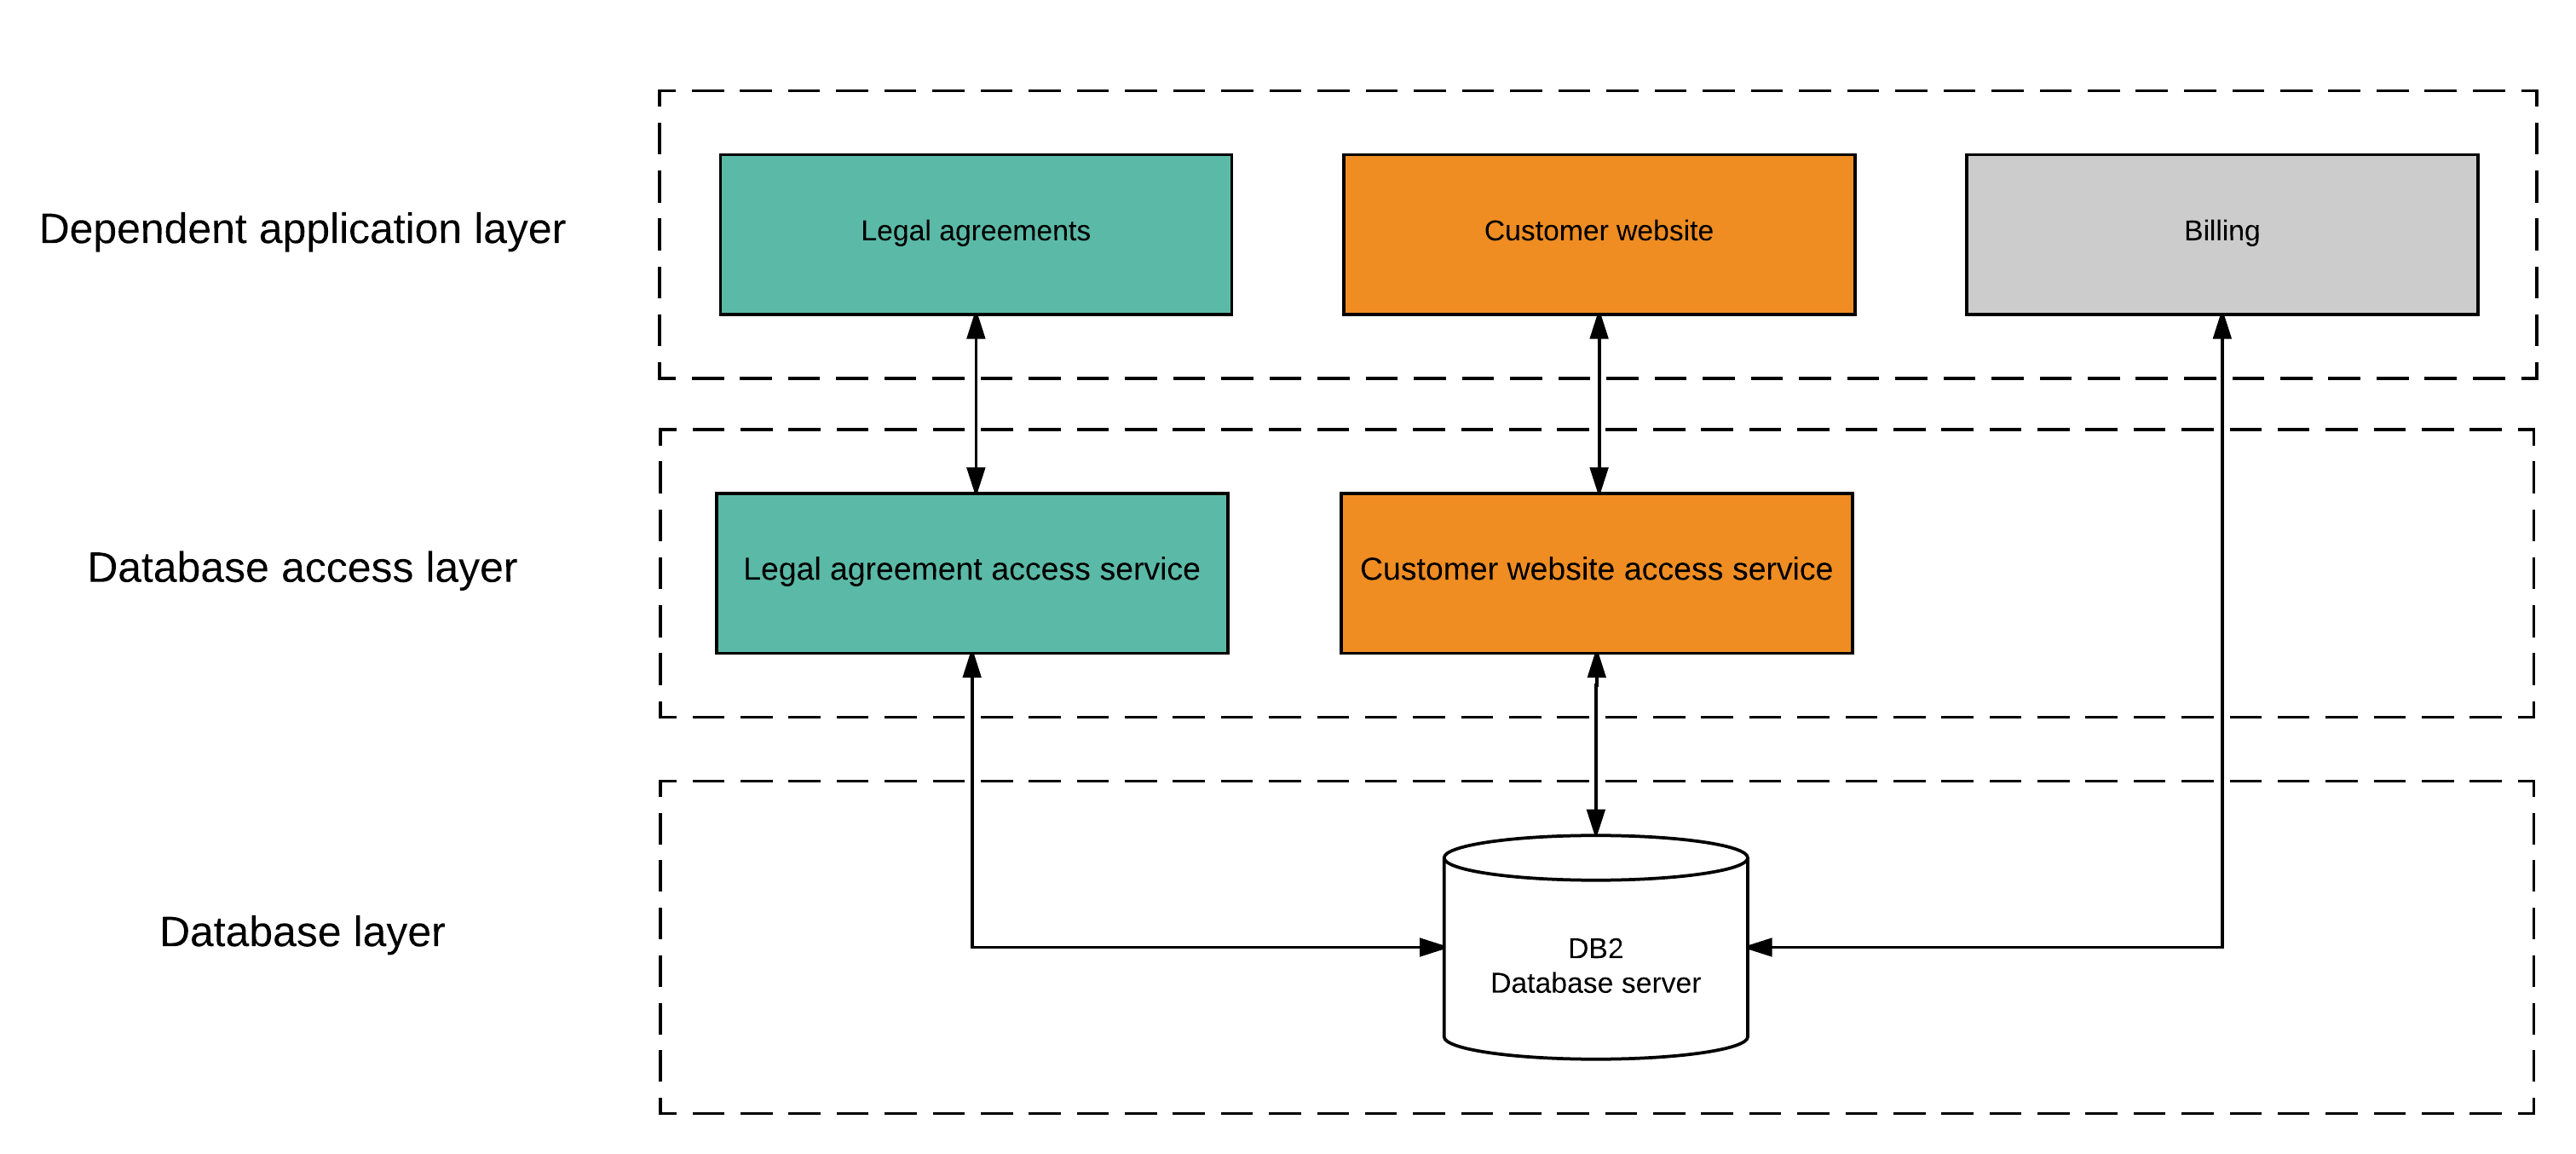
\includegraphics[width=\textwidth]{danske_bank_shared_database}  
  \caption{Datbase integration architecture}
  \label{fig:danske_bank_shared_database}
\end{figure}


Even though Danske Bank has tried to combat some of the issues with a shared database architecture, there is still inherently many problems and limitations with the architecture which will be further discussed in the following sections.

\section{The Shared Database}
This section will try to pin down why this form of integration has been so widespread, and secondly in greater detail which challenges and limitations it introduces. As hinted earlier, the shared database architecture is a very common integration method, but also a method filled with challenges. According to San Newman this form of integration is the most common one in enterprise applications \cite[p.~41]{newman2015microservices}. Martin Fowler also expresses how common this integration is, how he classifies the BCA architecture as being a Service Oriented Architecture (SOA) and the amount of problems this form of integration introduces \cite[t.~09:40]{fowler2014microservicesoamonolith}:

\tquote{... if we think about the monolithic world we think of the fact that generally all of the data is sitting in one honking big relational database ... everything goes in the same place and even in a lot of service oriented architectures it is really a lot about multiple services all pulling data in and out of one logical large database ... first it [referring to decentralization of data management in microservices] removes this horrible mess of integrating through a database, which causes no end of problems in enterprises all over the place ... }{Martin Fowler}{2014}. 

A database integration starts out very simple and is quickly established, but becomes rigid with time. Integration through a database is frowned upon by leading spokesmen writing literature and doing presentations about enterprise software architecture, presented as a mistake when Monolithic and SOA architectures were developed. There are many values of the relational database but also challenges when used as a shared relational database which will be described in detail below.

\subsection{The Value of the Relational Database}
There are several valuable aspects of utilizing a relational database, some of the main benefits are outlined below, followed by an explanation of why the relational database is wide use as an integration method.

\textbf{Persistent data}\\
Enterprise applications typically need some kind of data storage. There are several ways to store data, using either the filesystem or volative memory, but lack of flexibility and persistence makes these options less attractive. Databases introduce a flexible way to persist data with strong guarantees for concurrency \cite[p.~3]{sadalage2012nosql}.

\textbf{Concurrency}\\
Relational databases handle concurrency by providing data through transactions, containing most of the complexity when working with concurrency \cite[p.~4]{sadalage2012nosql}. 

\textbf{A Standard Model}\\
Good and basic standards for the utilization of relational databases makes it possible to use this type of databases very easily across different projects \cite[p.~4]{sadalage2012nosql}. 



Due to strong concurrency, a single database makes it possible to store and share data easily this is meant to be utilized internally in a single application, but can also easily be used across several applications, improving ease of communication \cite[p.~4]{sadalage2012nosql}. A single connection to the database can be reused within a dependant application, giving a single persistent reference to all relevant data.

\subsection{Challenges with a Shared Relational Database}
Challenges with a shared database in the BCA system and others alike can be divided into two groups: The limitations of relational databases, and database as an integration method.

\subsubsection{Limitations with Relational Databases}
The relational model is build around relations, hence the name, providing elegant relational algebra for writing and retrieving data, but at the same time it creates a difference between in-memory data structure and the database model, this is called \textit{Impedance Mismatch}. Moreover, the relational database model is inherently not designed to run on clusters, the only reasonable way to scale a relational database is vertically, creating a upper limit for the \textit{Capacity} and introducing a \textit{Single Point of Failure}, both described below. \comment{Cite fowler her}

\textbf{Single Point of Failure}\\
With a single point of failure each consumer is highly reliant on a correct and running database. All consumers are communicating with the same database, inferring a very high responsibility on each consumer, an incorrect implementation could cause the database to collapse, due to malformed or a high amount of requests from a single or several consumers, Nygaard includes this in his description of stability antipatterns \cite[p. 31]{nygard2007release}  (see section \ref{sec:stability_antipatterns}).
A high amount of applications are dependent on the singular database, and the lack of redundancy would cause a complete stop to the many applications dependent on the database if it was ever to crash, making any dependent service possibly unavailable.

\textbf{Capacity}\\
Two types of capacity scaling exists, vertical and horizontal. Vertical scaling incurs increasing the processing power on a singular server, while horizontal scaling incorporates replicating the application on several servers, relying less on individual server processing power by distributing load. With a single SQL database in place at the center of several applications, the capacity for these applications will be limited. Vertical scaling is limited to the biggest machine available, by choosing a architecture that only supports vertical scaling it will at some point be a limiting factor \cite[t.~08:30]{meshenberg2016microservices}.
Capacity improvement and the effects of replication is thoroughly investigated in chapter \ref{ch:implementation} section \ref{sec:Effects_of_Replication} where experiments have been conducted to show the effects of replication.

\subsubsection{Issues Sharing a Single Databases}

\textbf{High Coupling}\\
Each consumer without a database access layer is highly coupled to the database, making changes to the database structure incur changes in all directly linked consumer implementations.

\textbf{Loss of Cohesion}\\
By having several database access layers and dependent applications directly interacting with the database, the logic required to perform common operations on the database is duplicated. This infers a big overhead if a bug is discovered within this common logic, making it necessary to update several code bases with the same fix.

\textbf{Complex Model}\\
By sharing a database between several applications, the database needs to contain a richer model, incorporating all aspects needed by each involved applications. Creating a very complex model\cite[p.~6]{sadalage2012nosql}. Identifying what Eric Evans calls \textit{Bounded contexts} is extremely important to avoid several pitfalls (see section\ref{sec:DDD}).

\section{Summary}
There are inherently many problems with sharing a database between several services, and it should therefore be avoided. The main issues with this form of integration is the introduction of a single point of failure, incurring a big risk for depending services. Limiting the maximum amount of available capacity can also hurt availability, with a too low capacity, the database might get overloaded, completely coming to a halt or not responding on a certain percentage of the requests.

\comment{Jeg kan ikke skrue på de fire knapper i den her arkitektur, det er skod}